\documentclass[12pt, a4paper]{article}
\usepackage[utf8]{inputenc}
\usepackage[T2A]{fontenc}
\usepackage[english,russian]{babel}
\usepackage[usenames]{color}
\usepackage{hyperref}
\ifx\pdfoutput\undefined
\usepackage{graphicx}
\else
\usepackage[pdftex]{graphicx}
\fi

\title{Software Engineering from Innopolis}
\author{Vladimir Maximov}
\date{\today}

\begin{document}

\maketitle

\section{Итеритуемые объекты в Python}

\subsection{Цель}

Изучить коллекции в Python и работу с ними.

\subsection{Задачи}

\begin{itemize}
    \item Ознакомиться со списками в Python.
    \item Рассмотреть популярные операции, используемые
    над списками slice, filter, map, reduce.
    \item Ознакомиться с кортежем в Python.
    \item Разобрать различные подходы создания коллекций.
    \item Ознакомиться с множествами в Python.
    \item Понять, чем руководствоваться при выборе 
    коллекции для хранения объектов.
\end{itemize}

\subsection{Список}

Список - упорядоченная и изменяемая коллекция объектов:

\begin{verbatim}
1   my_list = [1, 2, 3, None, [0], "word"]
\end{verbatim}

Слайс (срез) списка - создание нового списка, 
используя элементы уже существующего:

\begin{verbatim}
1   my_list[2:4:1]
\end{verbatim}

Берем со 2 элемента включительно по 4 элемент 
невключительно с шагом 1.

% Это пропуск строки
\vspace{1em}

Краткая форма создания списка называется
List comprehention (генератор списка):
\begin{verbatim}
1   [x for x in range(10)]
\end{verbatim}

\subsection{Кортеж}

Кортеж - упорядоченная и неизменяемая коллекция:
\begin{verbatim}
1   (1, 2, 3, 4, 5)
\end{verbatim}

\subsection{Множество}

Множество - неупоярдоченная коллекция значений, 
в которой не допускаются повторения
и не может содержать не хешируемых объектов:
\begin{verbatim}
1   {1, 2, 3, "some string"}
\end{verbatim}

\subsection{Словари}

Словарь - изменяемая коллекция объектов, которые 
обладают ключевыми словами. В Python словарь можно
описать указанием ключей и значений элементов
или генерирующим выражением:
\begin{verbatim}
1   {"key1" : "value1",
2   "key2" : "value2",
3   "key3" : "value3"}
\end{verbatim} 

\subsection{Использование памяти}

Для хранения коллекций выделяется чуть больше памяти,
чем фактически необходимо. Делается это для того, 
чтобы интерпретатор Python при добавлении элементов
выделял память реже.

\vspace{1em}

В Python в коллекции можно хранить разные объекты, 
каждый из которых может быть непредвиданного размера.
Поэтому в Python в списке хранятся указатели на нужные объекты.

\subsection{Itertools}

itertools - модуль, который предоставляет различные функции 
для работы с итерируемыми объектами. Его можно использовать
для упрощения записи операций над итерируемыми объектами.
Примеры методов:

\vspace{1em}

itertools.combinations - метод для поиска подмножеств
итерируемого объекта, возвращает генератор: 
\begin{verbatim}
1   import itertools    
2   itertools.combinations("ABCD", 2)
3   list(itertools.combinations("ABCD", 2))
4   # Вывод: [(A, B), (A, C), (A, D), (B, C), (B, D), (C, D)]
\end{verbatim}

\vspace{1em}

itertools.compress - метод, который выбирает из исходного
итерируемого объекта элементы, согласно селектору (маске):
\begin{verbatim}
1   import itertools    
2   itertools.compress([1,2,3,4], [1,0,1,0])
3   list(itertools.compress([1,2,3,4], [1,0,1,0]))
4   # Вывод: [1,3]
\end{verbatim}
    
\vspace{1em}

\section{Функции над итерируемыми объектами}

\subsection{Цель}

Ознакомиться с тем, какие операции могут быть сделаны
на итерируемых объектах и что можно представить в качестве
итерируемого объекта.

\subsection{Задачи}

\begin{itemize}
    \item Ознакомиться как еще можно работать со списками
    \item На примерах понять, какие объекты можно представлять
    в качестве итерируемого объекта.
\end{itemize}

\subsection{Itertools (продолжение)}

Если стандартного набора библиотеки itertools не хватает,
то можно использовать сторонний пакет - 
\href{https://more-itertools.readthedocs.io/en/stable/api.html}
{\textcolor{blue}{more\textunderscore itertools}}, он расширяет
возможности работы с итерируемыми объектами. Примеры функций:

\vspace{1em}

Функция chunked:
\begin{verbatim}
1   from more_itertools import chunked
2   iterable = [0, 1, 2, 3, 4, 5, 6, 7, 8]
3   list(chunked(iterable, 3))
4   # Вывод: [[0, 1, 2], [3, 4, 5], [6, 7, 8]]
\end{verbatim}

Функция flatten:
\begin{verbatim}
1   from more_itertools import flatten
2   iterable = [(0, 1), (2, 3)]
3   list(flatten(iterable))
4   # Вывод: [0, 1, 2, 3]
\end{verbatim}

Функция split\textunderscore at:
\begin{verbatim}
1   from more_itertools import split_at
2   list(split_at('abcdcba', lambda x: x == 'b'))
3   # Вывод: [['a'], ['c', 'd', 'c'], ['a']]
\end{verbatim}

Функция transpose:
\begin{verbatim}
1   from more_itertools import transpose
2   list(transpose([(1, 2, 3), (11, 22, 33)]))
3   # Вывод: [['a'], ['c', 'd', 'c'], ['a']]
\end{verbatim}

Функция windowed:
\begin{verbatim}
1   from more_itertools import windowed
2   all_windows = windowed([1, 2, 3, 4, 5], 3)
3   list(all_windows)
4   # Вывод: [(1, 2, 3), (2, 3, 4), (3, 4, 5)]
\end{verbatim}

\subsection{Filter, Map, Reduce}

Иногда для целесообразного использования памяти лучше 
написать часть программы в функциональном стиле. 
Особенно это применимо когда нужно пройтись по большому 
количеству элементов. Для этого в python существуют встроенные
функции. Их использование будет рассмотрено на простых примерах.

\subsubsection{Filter}

Filter - функция, которая позволяет выбрать из любого 
итерируемого объекта элементы удовлетворяющие условию. 
В качестве аргумента принимает функцию или лямбда-выражение
и список, из которого отфильтрует значения:

\begin{verbatim}
1   items = [-5,-4,-3,-2,-1,0,1,2,3,4,5]
2   def my_filter_expr(item):
3       return item > 0
4   positive_items = tuple(filter(my_filter_expr, items))
5   print(positive_items)
6   # Вывод: (1, 2, 3, 4, 5)
\end{verbatim}

Важно понимать что получившийс объект не хранит в себе все 
элементы получившегося списка. Он хранит информацию о том 
как можно получить каждый из последующих элементов списка. 
Важно понимать как это работает чтобы в дальнейшем не попадать
на ошибки. Самый близкий родственный объект к получившемуся 
фильтру - итератор. Итератор это специальный объект в python 
который выдает по одном элементу и по нему можно пройтись 
только один раз.

\subsubsection{Map}

Map - функция, которая позволяет применить функцию ко всему 
списку значений. В качестве аргумента принимает функцию или 
лямбда-выражение и список, к элементам которого будет 
применена функция:

\begin{verbatim}
1   list(map(lambda a: a[0]**a[1], [(0, 2), (1, 2), (2, 2)]))
2   # Вывод: [0, 1, 4]
\end{verbatim}

\subsubsection{Reduce}

Reduce - функция, применяющая другую функцию к 
последовательным парам значений в списке, аналог функции
Fold в Wolfram Mathematica:

\begin{verbatim}
1   from functools import reduce
2   many_items = [1,2,3,4]
3   product = reduce(lambda a, b: a * b, many_items)
4   # Вывод: 24
\end{verbatim}

В начале в качестве переменной $a$ функция берет значение 1,
в качестве переменной $b$ - 2, на втором шаге переменная $a$ - 
результат функции на предыдущей итерации, $b$ - 3 и т.д. У
функции есть третий необязательный аргумент - начальное значение.

\subsection{Метод скользящего окна}

Метод скользящего окна представляет собой процесс, при котором 
окно фиксированного размера последовательно перемещается по 
набору данных. Значения внутри окна анализируются и 
обрабатываются для получения новых результатов, например, 
вычисления среднего или медианного значения.

\subsection{Операции из линейной алгебры}

Линейная алгебра это раздел математики, основными конструкциями
в которой являются списочный типы данных. Матрицы, векторы, 
тензоры - это все понятия из линейной алгебры.
Самые базовые математические операции в линейной алгебре - это 
операции на этих структурах определенных в линейном 
пространстве - транспонирование, перемножение матриц и 
векторов, нахождение определителей, решение системы 
линейныхуравнений. Пример перемнжения матриц в помощью
more\textunderscore itertools:

\begin{verbatim}
1   from more_itertools import matmul
2   matrix1 = [
3   [1,2,3],
4   [4,5,6],
5   ]
6   matrix2 = [
7   [7, 8],
8   [9, 10],
9   [11, 12],
10  ]
11  list(matmul(matrix1, matrix2))
12  # Вывод: [[58, 64], [139, 154]]
\end{verbatim}

\newpage

\subsection{Линейная алгебра с numpy}

numpy - библиотека, которая заточена под выполнение 
операций на матрицах. Основные фукнции можно посмотреть по 
\href{https://github.com/KeithGalli/NumPy/blob/master/
NumPy%20Tutorial.ipynb}{\textcolor{blue}{ссылке}}. 
Пример перемножения матриц с помощью numpy:

\begin{verbatim}
1   import numpy as np
2   matrix1 = np.array([
3   [1,2,3],
4   [4,5,6],
5   ])
6   matrix2 = np.array([
7   [7, 8],
8   [9, 10],
9   [11, 12],
10  ])
11  matrix1 @ matrix2
12  # Вывод: array([[58, 64], [139, 154]])
\end{verbatim}

\section{Базы данных и SQL, работа с бд 
из Python}

\subsection{Цель}

Рассмотреть базы данных как один из 
возможных источников данных для работы.

\subsection{Задачи}

\begin{itemize}
    \item Разобраться как работать с табличными 
    данными
    \item Понять, как можно обращаться с табличными
    данными из python
    \item Выяснить, каким инстументарием можно 
    воспользоваться для работы с табличными данными.
\end{itemize}

\subsection{Табличное представление данных, 
именованные данные, работа с ними}

Когда мы работае с данными, часто так бывает 
что они представлены в виде таблиц. То есть 
представлят собой последовательные наборы строк 
с данными, в которой каждый отдельный элемент 
может быть ассоциирован с наименованием и/или 
типом данных.


\subsection{Реляционные базы данных}
Табличное представление свойственно для 
реляционных БД. База данных (БД) - 
это специальным образом организованная 
совокупность данных о некоторой предметной 
области, хранящаяся во внешней памяти компьютера.
В таких таблицах все поля не только уникально 
проименованы, но и имеют строгий тип данных, 
а также могут иметь ограничения по уникальности 
и связи с другими таблицами.
Пройденный курс по SQL с заданиями в СУБД 
MySQL по \href{https://sql-academy.org/ru/guide}
{\textcolor{blue}{ссылке}}.

\subsection{Работа из python: sqlite3, 
psycopg2, pandas}

Для работы с данными из реляционных БД в языке 
программирования python существуют библиотеки 
для низкоуровневого взаимодействия с ними.
Для связи с БД sqlite, кторая не запускается на 
отдельном сервере а хранится файлом в 
локальной файловой системе, существует модуль 
sqlite3, который не нужно устанавливать отдельно, 
он встроен в стандартную библиотеку python.
В его стандартный функционал входит соединение с базой, 
исполнение sql выражений и работа с полученным от 
резаультата выражением как с объектом знакомым 
языку программирования (итерируемый объект).
\begin{verbatim}
1     import sqlite3
2     from contextlib import closing
3 
4     sqlite_filename = "datasets/movies.sqlite"
5     con = sqlite3.connect(sqlite_filename)
6     def dict_factory(cursor, row):
7         d = {}
8         for idx, col in enumerate(cursor.description):
9             d[col[0]] = row[idx]
10        return d
11    
12    con.row_factory = dict_factory
13
14    with closing(con.cursor()) as cur:
15        for row in cur.execute("SELECT * FROM movies JOIN\ 
16        \directors ON movies.director_id = directors.id"):
17            print(row)
\end{verbatim}
В данном случае мы с использованием sqlite3 получаем все
фильмы из таблицы \(movies\), режиссеры которых присутствуют 
в таблице \(directors\).  

\vspace{1em}

Самым классическим инструментом для работы с датасетами 
является pandas. Помимо того чтобы работать с данныими из 
электронных таблиц, он может забрать данные из sql-query, 
если в качестве параметра ему передать соединение с базой.
Данные, полученные с помощью sql select можно сразу же 
загрузить в датафрейм. у pandas есть такой инструмент.

\begin{verbatim}
1    import pandas as pd
2    import pandas.io.sql as psql
3
4    connection = psycopg2.connect("dbname=test user=student1\
5    \password=student1 host=212.109.218.158 port=5432")
6    dataframe = psql.read_sql('SELECT * FROM files JOIN\
7    \person ON files.owner = person.id;', connection)
\end{verbatim}

\subsection{Краткое объяснение нереляционных баз данных \
на примере MongoDB}

Не все БД занимаются хранением связанных прямоугольных таблиц. 
Это происходит потому что тип хранилища состоящий из строго 
типизорованных связанных таблиц подзодит не для всех типов задач.
Один из примеров такой базы - MongoDB.

\vspace{1em}

Mongo - популярная хостируемая на сервере документная 
(не реляционная, NoSQL) БД. Структура данных в этой и 
подобных базах отличается от всего пройденного до этого.
Напоминает словари в python или же json файл.
Причинами выбора именно нереляционной базы для вашего 
проекта могут быть следующие:

\begin{itemize}
    \item В проекте (или его части) не нужны взаимоотношения 
    между объектами, вы собираетесь хранить много данных в 
    коллекции, каждый объект в которой самостоятелен сам по 
    себе. Часто это фронтенд-ориентированные проекты или части 
    проектов. (отсутствие связей между объектами и быстрый поиск 
    по коллекции позволяют быстро выдавать данные для 
    отображения на сайте или мобильном устройстве)
    \item Заранее не известна модель хранимых данных 
    \item Отличная масштабируемость
\end{itemize}

\section{numpy / pandas}

\subsection{Цель}

Ознакомиться с функционалом основного инструмента анализа данных.

\subsection{numpy}

Самый фундаментальный \href{https://numpy.org/}
{\textcolor{blue}{пакет}} для работы с данными. Часто он 
выступает основой для других пакетов работы с данными. В 
частности это происходит потому что разработчики библиотеки 
на очень глубинном уровне переработали взаимедействие python 
с коллекциями (особенно многомерными). В результате чего 
работа с numpy.ndarray происходит значительны быстрее по 
скорости чем со стандартным list.

\vspace{1em}

Основной пакет, который будет использоваться - 
\href{https://numpy.org/doc/stable/reference/routines.linalg.html}
{\textcolor{blue}{numpy.linalg}}. Все алгоритмы, связанные 
с линейной алгеброй есть в данном пакете.

\subsection{pandas}

Обычно при работе с данными мы наблюдаем что каждый кусочек 
данных помимо числовых значений может относиться к разным 
категориям, быть логически отделимым от другого куcочка таких 
же данных по набору признаков. Тут для анализа данных 
появляется такой инструмент как 
\href{https://pandas.pydata.org/docs/getting_started/index.html}
{\textcolor{blue}{pandas}}. Он реализует работу 
с кусками данных. Тип объекта с данными который загружен 
с помощью pandas будет называтья DataFrame, а одна отдельная 
запись из датафрейма будет называться series.

\vspace{1em}

Внутри себя pandas использует алгебру реализованную в NumPy.
pandas имеет под собой зависимость в numpy. 

\vspace{1em}

\textbf{Series} (серия)- это одномерный, именованный (помеченный) массив, 
который может хранить данные любого типа, включая целые числа, 
числа с плавающей точкой, строки и объекты Python. Базовая 
структура серии состоит из двух компонентов: данных и индекса.
В серии данные представляют собой одномерный массив NumPy, 
содержащий фактические значения данных.

\newpage

\begin{verbatim}
1     data_frame_covid.T.iloc[:,0]
2     # Вывод:
3     # country         Afghanistan
4     # continent              Asia
5     # date             2020-04-12
6     # day                      12
7     # month                     4
8     # year                   2020
9     # cases                    34
10    # deaths                    3
11    # country_code            AFG
12    # population       37172386.0
13    # Name: 0, dtype: object

14    type(data_frame_covid.T.iloc[:,0])
15    # Вывод: pandas.core.series.Series
\end{verbatim}

\textbf{Индекс} - это структура, похожая на массив, которая помечает 
каждый элемент массива данных. По умолчанию индекс представляет 
собой последовательность целых чисел, начинающуюся с нуля, но 
также можно предоставить пользовательские метки для индекса. 
Это облегчает обращение и манипулирование элементами данных на 
основе их меток. Чтобы создать серию, можно использовать 
конструктор pd.Series() и передать список, словарь или массив 
NumPy в качестве данных. Также можно передать необязательный 
параметр индекса, чтобы указать пользовательские метки для 
элементов данных.

\vspace{1em}

\textbf{DataFrame} (ДатаФрейм, Таблица данных) - это двумерная, 
изменяемая в размере и гетерогенная структура табличных данных 
с маркированными осями (строками и столбцами). Его можно 
рассматривать как коллекцию объектов Series, где каждый 
столбец представляет собой объект Series. DataFrames 
предназначены для обработки широкого спектра типов данных, 
что делает их универсальным и мощным инструментом для обработки 
и анализа данных. Базовая структура DataFrame состоит из трех 
компонентов: данных, индекса и столбцов.
В DataFrame данные хранятся в виде коллекции из одного или 
нескольких объектов Series, каждый столбец которых представляет 
собой отдельную Series. Данные в каждой Series могут быть 
различных типов, таких как целые числа, числа с плавающей точкой 
или строки.

\vspace{1em}

\textbf{Столбцы} являются структурой, подобной массиву, которая 
помещает метку на каждый столбец в DataFrame.

\begin{verbatim}
1   data_frame_covid.columns
2   # Вывод: Index(['country', 'continent', 'date', 'day', 
3   #       'month', 'year', 'cases',
3   #       'deaths', 'country_code', 'population'],
4   #       dtype='object')
\end{verbatim}

Как Series так и DataFrame предоставляют методы для анализа 
данных, такие как:

\begin{itemize}
    \item Выборка данных: можно указать особые строки и колонки 
    с которыми вы будете работать, используя индексы, слайсы, 
    условия
    \item Очистка данных: можно заполнять пропущенные данные, 
    удалять записи в которых не хватает данных.
    \item Преобразование данных: можно применять функции по всей 
    длинне фрейма или по его отдельным частям
    \item Аггрегация данных: можно вычислять такие оценочные 
    величины как сумма, среднее, количество.А также группировать 
    данные по своим критериям при помощи groupby.
    \item Сортировка: можно упорядочить данные основываясь на 
    значениях в колонках, а также по своим критериям
    \item Функциональность временных рядов: вы можете работать 
    с данными временных рядов, пересчитывать данные с разной 
    частотой и выполнять вычисления с использованием скользящего 
    окна в DataFrame или Series.
\end{itemize}

В качестве основных типов данных для работы, pandas использует 
типы данных из NumPy по пораву наследования, ознакомиться с 
которыми можно по \href{https://pandas.pydata.org/pandas-docs/
stable/reference/arrays.html}{\textcolor{blue}{ссылке}}.

\vspace{1em}

Во многом успех работы с данными зависит в скорости доступа 
к данным и возможности быстро отфильтровать ненужное. Для 
ускорения работы нам могут помочь индексы. При создании 
датафрейма у него имеется стандартный индекс для быстрого 
доступа через него до строк данных. Выбирать такие строки 
можно с помощью функций \(.loc()\) и \(.iloc()\) (i==integer). Для 
датафрейма можно установить новый индекс (при этом либо 
заменив старый либо создав новый датафрейм из существующего 
с новым индексом).

\newpage

Комбинирование фреймов:
\begin{verbatim}
1   data_frame_covid[1:3]
2       .append(data_frame_covid[-3:-1], ignore_index=True)    
\end{verbatim}

\begin{figure}[h]
    \begin{center}
        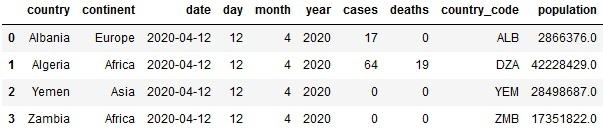
\includegraphics[scale=0.5,keepaspectratio]
        {Pictures/Picture_1.jpg}
        \caption{результат комбинирования фреймов}
        \label{Picture_1}
    \end{center}
\end{figure}

Для того чтобы выбрать несколько условий для фильтрации 
датафрейма можно воспользоваться методом query(), он 
позволяет в одну строку записать все условия фильтрации 
которые вам могут быть нужны при выборе данных. при этом 
в результате вы получите новый фрейм с данными.
\begin{verbatim}
1   data_frame_covid.query("cases > 5")
\end{verbatim}

\begin{figure}[h]
    \begin{center}
        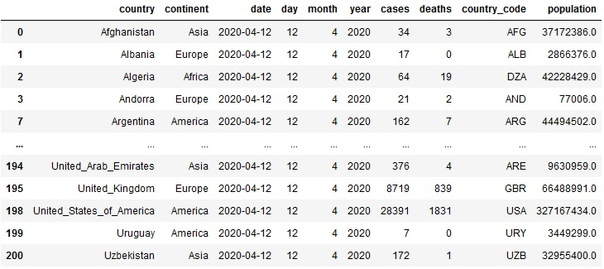
\includegraphics[scale=0.5,keepaspectratio]
        {Pictures/Picture_2.jpg}
        \caption{фильтрация фрейма}
        \label{Picture_2}
    \end{center}
\end{figure}

\section{Разведывательный анализ данных}

\subsection{Цель}

Научиться понимать, описывать набор данных c помошью 
инструментов на языке программирования python.

\subsection{Смысл разведывательного анализа данных}

Когда мы работаем с небольшими данными, мы хотя бы в 
общих чертах понимаем основные характеристики датафрейма: 
сколько в нем данных, насколько одни разнородны, что их 
объединяет, могут ли быть колонки связаны друг с другом.

\begin{verbatim}
1    data = {
2        'Name': ['Вася', 'Коля', 'Маша', 'Сережа'], 
3        'Age': [20, 21, 19, 18],
4        'Height': [183, 176, 163, 180],
5    } 
6    
7    simple_data_frame = pd.DataFrame(data) 
8    simple_data_frame
\end{verbatim}

\begin{figure}[h]
    \begin{center}
        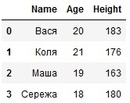
\includegraphics[keepaspectratio]
        {Pictures/Picture_3.jpg}
        \caption{небольшой датафрейм}
        \label{Picture_3}
    \end{center}
\end{figure}

Для начала работы с большими фреймами есть разведывательный 
анализ данных (Exploratory Data Analysis, EDA). Это набор 
техник работы с данными, позволяющий, если кратко говорить, 
ответить на вопрос "что передо мной такое, с чем я работаю?". 
Вопрос звучит просто, однако он требует умения работы со 
статистикой, понимания соответствующих терминов. Также вопрос 
усложняется тем что на него существует одновременно большое 
множество правильных ответов и чем больше вы исследуете датасет 
тем больше верных утверждений вы на него обнаружите.

\newpage

Для описания датафрейма в целом есть метод \(info()\):

\begin{verbatim}
1    data_frame.info()
\end{verbatim}

\begin{figure}[h]
    \begin{center}
        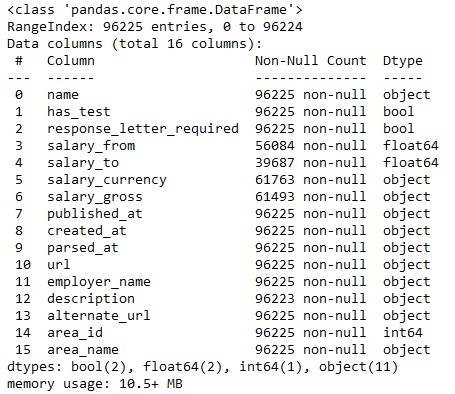
\includegraphics[scale=1,keepaspectratio]
        {Pictures/Picture_4.jpg}
        \caption{результат метода info()}
        \label{Picture_4}
    \end{center}
\end{figure}

Самое первое что стоит сделать до математических оценок 
чего бы то ни было - это проверить, 
наколько пуст наш набор данных. 
Есть вероятность что во множестве критически важных 
колонок нашего датасета вписаны пустые значения и тогда 
ценность для нас такого набора данных резко снижается.

\newpage

\begin{verbatim}
1    data_frame.isna().sum()
\end{verbatim}

\begin{figure}[h]
    \begin{center}
        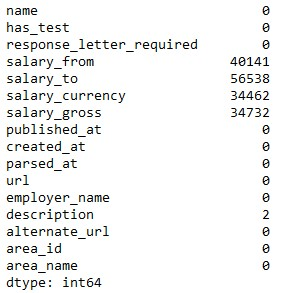
\includegraphics[scale=1,keepaspectratio]
        {Pictures/Picture_5.jpg}
        \caption{наполненность датасета}
        \label{Picture_5}
    \end{center}
\end{figure}

\subsection{Оценка центрального положения}

Базовый шаг любого развед-анализа (одно из первых действий 
которое вы выполняете) это определение среднего положения. 
То есть ответ на вопрос "как выглядит самое типичное значение 
в моих данных?". То есть оценка того, где расположено 
большинство данных (центральная тенденция). При этом не всегда 
взятие "среднего арифметического" это самый правильный подход 
к такой оценке. А вдруг мой набор данных содержит странные 
выбросы самого наибольшего и наименьшего значния? А откуда я 
вообще знаю что такое среднее чувствительно к выбросам?
Для того чтобы получить "самое среднее" среднее есть 
различные методы.

\newpage

\begin{verbatim}
1    data_frame.describe()[critical_columns_numeric]
\end{verbatim}

\begin{figure}[h]
    \begin{center}
        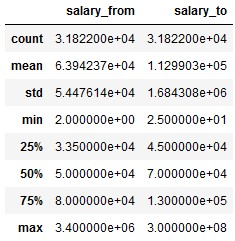
\includegraphics[scale=1,keepaspectratio]
        {Pictures/Picture_6.jpg}
        \caption{наполненность датасета}
        \label{Picture_6}
    \end{center}
\end{figure}

Оценки:
\begin{itemize}
    \item mean - среднее - среднее арифметическое - самая 
    примитивная оценка центрального положения.
    \item Средневзвешенное - вычисляется как сумма значений 
    умноженная на веса, деленная на сумму весов. Такая оценка 
    среднего положения предполагает наличие колонки с весами, 
    то есть некоего коэффицианта, показывающего что значение 
    из одной строчки ценятся чуть больше чем значение из другой.
    \item Среднеусеченное - это такое среднее значение 
    которое вычисляется после отсечения предельных значений. 
    Такое понимание среднего позволяет обрезать "хвосты" 
    распределения (что не всегда уместно, особенно при резком 
    перекосе асимметрии распределения). 
    \item Медиана (50й процентиль, 0,5-квантиль, Q2) - значение, 
    которое находится в середине упорядоченного набора данных.
    \item Мода - наиболее часто встречающаяся категория или 
    значение в наборе данных. 
\end{itemize}

\subsection{Оценка вариабельности}

Вариабельность (дисперсность, variance) показывает насколько 
наборы данных расположены плотно друг к другу. Из оценок на 
основе дисперсности можно выяснить насколько строки данных 
логически близки друг к другу, то есть сделать вывод либо 
"данные слишком разнородны чтобы их как-то ообщать" либо 
"подавляющее большинство данных кучкуется вместе в пределах 
таких-то значений".

\vspace{1em}

Самый первый количественный показатель тут это стандартное 
отклонение. Оно говорит насколько данные в наборе в целом 
разросаны от центрального значения.

$$s = \sqrt\frac{\sum (x - \bar{x}) ^2}  {n-1} $$

\begin{verbatim}
1    data_frame.std(numeric_only=True)
\end{verbatim}

\begin{figure}[h]
    \begin{center}
        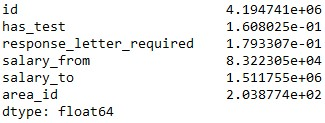
\includegraphics[scale=1,keepaspectratio]
        {Pictures/Picture_7.jpg}
        \caption{оценка вариабельности}
        \label{Picture_7}
    \end{center}
\end{figure}

Среднее абсолютное отклонение (mean absolute deviation) - 
среднее абсолютных значений отклонений от среднего, 
имеет смысл использоать в случае большого числа "выбросов", 
поскольку в отличие от std(), mad() к ним менее чувствителен.

$$\bar{d} = \frac{\sum_{i=1}^{n} \mid x_i - \bar{x} \mid }  {n} $$

Статистические показатели на основе сортированных (ранжированных) 
данных называются порядковыми статистиками. Элементарная мера — 
это размах: разница между самым крупным и самым малым значеними.
Во избежание чувствительности к выбросам вы можете обратиться к 
размаху данных после отбрасывания значений с каждого конца. Эти 
типы оценок формально основываются на разницах между 
процентилями. В наборе данных P-й процентиль является таким 
значением, что, по крайней мере, P процентов значений принимает 
это значение или меньшее, и по крайней мере (100 - P) процентов 
значений принимает это значение или большее.

\subsection{Оценки распределения}

Разведывание распределения данных показывает как данные 
расположены в совокупности. Здесь активно используются 
визуальные инструменты.

\vspace{1em}

В статистической теории центральное положение и вариабельность 
упоминаются как моменты распределения первого и второго порядка. 
Моменты третьего и четвертого порядка — это асимметрия и эксцесс.

\vspace{1em}

Асимметрия (skewness) - это мера асимметрии распределения. Это 
значение может быть положительным или отрицательным.

\begin{itemize}
    \item Отрицательная асимметрия указывает на то, что хвост 
    находится в левой части распределения, которая простирается 
    в сторону более отрицательных значений.
    \item Положительная асимметрия указывает на то, что хвост 
    находится на правой стороне распределения, которая 
    простирается в сторону более положительных значений.
    \item Нулевое значение указывает на то, что в распределении 
    вообще нет асимметрии, что означает, что распределение 
    совершенно симметрично.
\end{itemize}

\vspace{1em}

Эксцесс (kurtosis) - это мера того, является ли распределение 
тяжелым или легким хвостом по сравнению с нормальным 
распределением.

\begin{itemize}
    \item Эксцесс нормального распределения равен 3.
    \item Если данное распределение имеет эксцесс меньше 3, 
    говорят, что оно является игровым , что означает, что 
    оно имеет тенденцию производить меньше и менее экстремальных 
    выбросов, чем нормальное распределение.
    \item Если данное распределение имеет эксцесс больше 3, 
    говорят, что оно лептокуртическое , что означает, что оно 
    имеет тенденцию производить больше выбросов, чем нормальное 
    распределение.
\end{itemize}

\subsection{Matplotlib}

Один из инструментов визуализации позволяет строить различные 
двухмерные и трехмерные графики. Очень хорошо подходит для 
статистики. Большинство статистической визуализации которое 
вы увидите при изучении темы где-то в интернете обычно 
сделано либо через 
\href{https://matplotlib.org/}{\textcolor{blue}{matplotlib}} 
либо через seaborn, иногда с 
использованием bokeh.

\subsection{boxplot}

\href{https://builtin.com/data-science/boxplot}
{\textcolor{blue}{Коробчатая диаграмма}} (иногда в русскоязычной 
литературе называется "коробка с усами") позволяет наглядно 
продемонстрировать плотноть распеределения данных. Она 
основана на процентилях, то есть показывает выше и 
ниже какого уровня распределен набор значений. На ней 
показываются медианное значение - линия посередине коробки, 
75 и 25 процентили - верхняя инижняя граница коробки (IQR), 
"усы" коробки обозначают "максимумы" и "минимумы" набора 
данных, а точками обозначаются "выбросы" - те значения, 
встретить которые маловерятно.

\begin{figure}[h]
    \begin{center}
        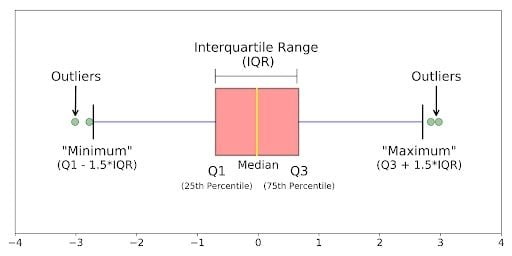
\includegraphics[scale=0.75,keepaspectratio]
        {Pictures/Picture_8.jpg}
        \caption{коробчатая диаграмма}
        \label{Picture_8}
    \end{center}
\end{figure}

\newpage

\subsection{histogram}

Гистограмма относится к частоте появления переменных в интервале.

\begin{verbatim}
1    data_frame[column_of_interest]
2        .value_counts()
3        .nlargest(40)
4        .plot(kind='bar', figsize=(15,5)) 
5        # nlargest(x) возвращает x наибольших значений.
6    plt.title("Частота предложений по зарплате")
7    plt.ylabel('Число предложений')
8    plt.xlabel('Salary from')
\end{verbatim}

\begin{figure}[h]
    \begin{center}
        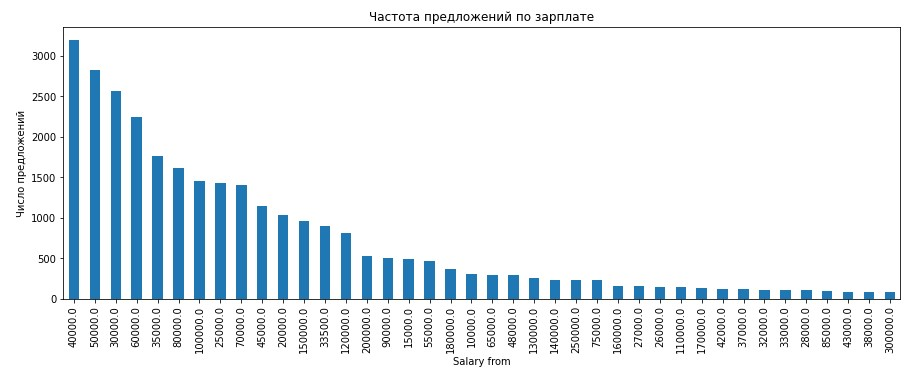
\includegraphics[scale=0.5,keepaspectratio]
        {Pictures/Picture_9.jpg}
        \caption{гистограмма}
        \label{Picture_9}
    \end{center}
\end{figure}

\newpage

\subsection{Корреляция}

Развед анализ также предполагает выяснение зависимости 
между исследуемыми переменными.
Матрица корелляции - один из основных способов понять 
взаимосвязь между переменными.

\begin{verbatim}
1    plt.figure(figsize=(10,5))
2    c = data_frame[[column_of_interest, "salary_to", "area_id"]]
3    .corr()
4    sns.heatmap(c, cmap="BrBG", annot=True)
\end{verbatim}

\begin{figure}[h]
    \begin{center}
        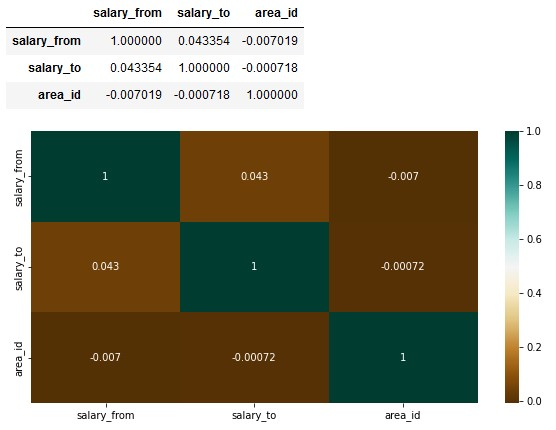
\includegraphics[scale=0.5,keepaspectratio]
        {Pictures/Picture_10.jpg}
        \caption{матрица корреляции}
        \label{Picture_10}
    \end{center}
\end{figure}

\end{document}